% !TeX root = ../../thesis.tex
\chapter{Algebraic Expressions for the Dyson Orbitals}\label{ch:appendix:dyson}

\subsubsection{EOM-EA-CC Dyson orbitals}
Right EOM-EA-CC Dyson orbital, $\phi^\mathrm{EA,R}_\mathrm{D} = \sum_i^\mathrm{occ} \gamma^\mathrm{EA,R}_i \phi_i + \sum_a^\mathrm{vir} \gamma^\mathrm{EA,R}_a \phi_a$:
\noindent\begin{flalign}
    \qquad \gamma^\mathrm{EA,R}_{i} &= \langle EA | \hat{a}^{\dagger}_i | CC \rangle & \\ 
    & = l_a \\
    \gamma^\mathrm{EA,R}_{a} &= \langle EA | \hat{a}^{\dagger}_a | CC \rangle \notag \\
    & = - \sum_c t_{ic} l_c - \frac{1}{2} \sum_{kcd} t_{ki}^{dc} l_{dc}^k
\end{flalign}

Left EOM-EA-CC Dyson orbital, $ \phi^\mathrm{EA,L}_\mathrm{D} = \sum_i^\mathrm{occ} \gamma^\mathrm{EA,L}_i \phi_i + \sum_a^\mathrm{vir} \gamma^\mathrm{EA,L}_a \phi_a$:
\noindent\begin{flalign}
    \qquad \gamma^\mathrm{EA,L}_{i} &= \langle CC | \hat{a}_i | EA \rangle \notag & \\ 
    & = - \sum_c \lambda_{ic} r_{c} - \frac{1}{2} \sum_{kcd} \lambda_{ik}^{cd} r_{k}^{dc} \\
    \gamma^\mathrm{EA,L}_{a} &= \langle CC | \hat{a}_a | EA \rangle \notag \\
    & = r_a + \sum_{kc} \lambda_{kc} r_{ca}^k + \sum_k \gamma^\mathrm{EA,L}_k t_{ka} - \frac{1}{2} \sum_{klcd} \lambda_{lk}^{dc} t_{lk}^{da} r_{c}
\end{flalign}

\subsubsection{EOM-EA-EE-CC Dyson orbitals}
Right Dyson orbital, $ \phi^\mathrm{EA-EE,R}_\mathrm{D} = \sum_i^\mathrm{occ} \gamma^\mathrm{EA-EE,R}_i \phi_i + \sum_a^\mathrm{vir} \gamma^\mathrm{EA-EE,R}_a \phi_a $:

\noindent\begin{flalign}
    \qquad \gamma^\mathrm{EA-EE,R}_{i} &= \langle EA | \hat{a}^{\dagger}_i | EE \rangle \notag & \\
    & = r_0 \gamma^\mathrm{EA,R}_a - \sum_c r_{ic} l_c - \frac{1}{2} \sum_{lcd} r_{il}^{cd} l_{dc}^l - \sum_{lcd} l_{dc}^l t_{ic} r_{ld} \\
    \gamma^\mathrm{EE-EA,R}_{a} &= \langle EA | \hat{a}^{\dagger}_a | EE \rangle \notag &\\
    & = r_0 l_a + \sum_{kc} l_{ca}^k r_{kc}
\end{flalign}

Left Dyson orbital, $ \phi^\mathrm{EE-EA,L}_\mathrm{D} = \sum_i^\mathrm{occ} \gamma^\mathrm{EE-EA,L}_i \phi_i + \sum_a^\mathrm{vir} \gamma^\mathrm{EE-EA,L}_a \phi_a$:
\noindent\begin{flalign}
    \qquad \gamma^\mathrm{EE-EA,L}_{i} &= \langle EE | \hat{a}_i | EA \rangle \notag & \\
    & = - \sum_c l_{ic}r_{c} - \frac{1}{2} \sum_{kcd} l_{ik}^{cd} r_{k}^{dc} \\ 
    \gamma^\mathrm{EE-EA,L}_{a} &= \langle EE | \hat{a}_a | EA \rangle \notag \\
    & = \sum_{kc} l_{kc}r_{ca}^k + \sum_k \gamma^\mathrm{EE-EA,L}_k t_{ka} - \frac{1}{2} \sum_{klcd} l_{lk}^{dc} t_{lk}^{da} r_{c}
\end{flalign}

\subsubsection{EOM-IP-CC Dyson orbitals}
Right Dyson orbital, $ \phi^\mathrm{EE,R}_\mathrm{D} = \sum_i^\mathrm{occ} \gamma^\mathrm{IP,R}_i \phi_i + \sum_a^\mathrm{vir} \gamma^\mathrm{IP,R}_a \phi_a $:

\noindent\begin{flalign}
    \qquad     \gamma^\mathrm{IP,R}_{a} &= \langle CC | \hat{a}^{\dagger}_a | IP \rangle \notag \\
    &= \lambda_{ka}r_{k} + \frac{1}{2} \lambda_{lk}^{ca} r_{klc} \\
    \gamma^\mathrm{IP,R}_{i} &= \langle CC | \hat{a}^{\dagger}_i | IP \rangle \notag & \\
    &= r_i + \sum_{kc} \lambda_{kc}r_{ik}^c - \sum_c \gamma^\mathrm{IP,R}_c t_{ic} - \frac{1}{2} \sum_{klcd} \lambda_{lk}^{dc} t_{li}^{dc} r_{k}
\end{flalign}

Left Dyson orbital, $ \phi^\mathrm{IP,L}_\mathrm{D} = \sum_i^\mathrm{occ} \gamma^\mathrm{IP,L}_i \phi_i + \sum_a^\mathrm{vir} \gamma^\mathrm{IP,L}_a \phi_a$:
\noindent\begin{flalign}
    \qquad     \gamma^\mathrm{IP,L}_{i} &= \langle IP | \hat{a}_i | CC \rangle \notag \\
    &= l_i \\
    \gamma^\mathrm{IP,L}_{a} &= \langle IP | \hat{a}_a | CC \rangle \notag & \\
    &= \sum_k t_{ka} l_k + \frac{1}{2} \sum_{klc} t_{kl}^{ac} l_{kl}^c
\end{flalign}

\subsubsection{EOM-EE-IP-CC Dyson orbitals}
Right Dyson orbital, $ \phi^\mathrm{EE-IP,R}_\mathrm{D} = \sum_i^\mathrm{occ} \gamma^\mathrm{EE-IP,R}_i \phi_i + \sum_a^\mathrm{vir} \gamma^\mathrm{EE-IP,R}_a \phi_a $:

\noindent\begin{flalign}
    \qquad \gamma^\mathrm{EE-IP,R}_{i} &= \langle EE | \hat{a}^{\dagger}_i | IP \rangle \notag  &\\
    &= \sum_{kc} l_{kc}r_{ik}^c - \sum_c \gamma^{IP-EI}_c t_{ic} - \frac{1}{2} \sum_{klcd} l_{lk}^{dc} t_{li}^{dc} r_{k} \\
    \gamma^\mathrm{EE-IP,R}_{a} &= \langle EE | \hat{a}^{\dagger}_a | IP \rangle \notag \\
    &= l_{ka}r_{k} + \frac{1}{2} l_{lk}^{ca} r_{klc}
\end{flalign}

Left Dyson orbital, $\phi^\mathrm{IP-EE,L}_\mathrm{D} = \sum_i^\mathrm{occ} \gamma^\mathrm{IP-EE,L}_i \phi_i + \sum_a^\mathrm{vir} \gamma^\mathrm{IP-EE,L}_a \phi_a$:
\noindent\begin{flalign}
    \qquad \gamma^\mathrm{IP-EE,L}_{i} &= \langle IP | \hat{a}_i | EE \rangle \notag & \\
    &= r_0 l_i + \sum_{kc} l_{ik}^c r_{kc} \\
    \gamma^\mathrm{IP-EE,L}_{a} &= \langle IP | \hat{a}_a | EE \rangle \notag \\
    &= r_0 \gamma^\mathrm{IP,L}_a + \sum_k r_{ka} l_k + \frac{1}{2} \sum_{klc} r_{kl}^{ac} l_{kl}^c + \sum_{klc} l_{kl}^c t_{ka} r_{cl}
\end{flalign}

\chapter{Photoelectron Cross-sections}\label{ch:appendix:crosssection}

\centering
\subsection*{Sample Jobs from \textit{ezDyson} Package}
\vfill
\ch{CH2}, SF to IP [\ch{CH2} ($^1$A$_1$) $\to$ \ch{CH2+} ($^2$A$_1$)], Basis set: 6-31G*
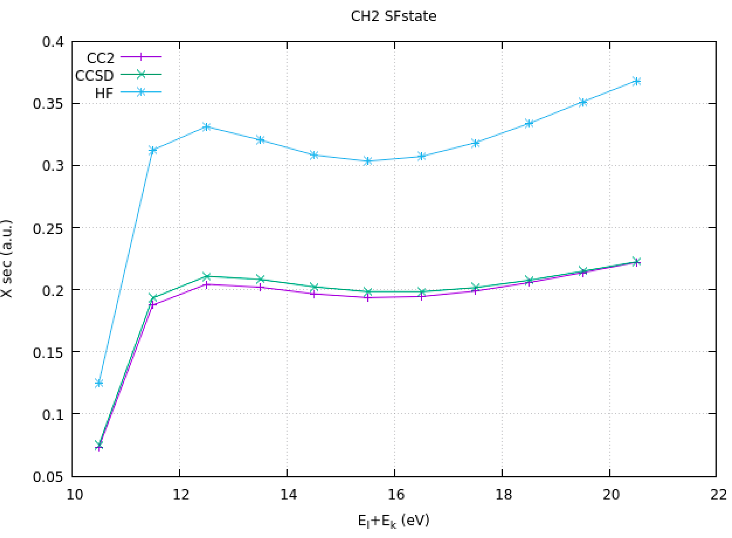
\includegraphics[width=0.6\textwidth]{chapters/appendix/image/Picture1.png}\\
\vfill
Formaldehyde, GS(HOMO)-IP, basis set: 6-31G*
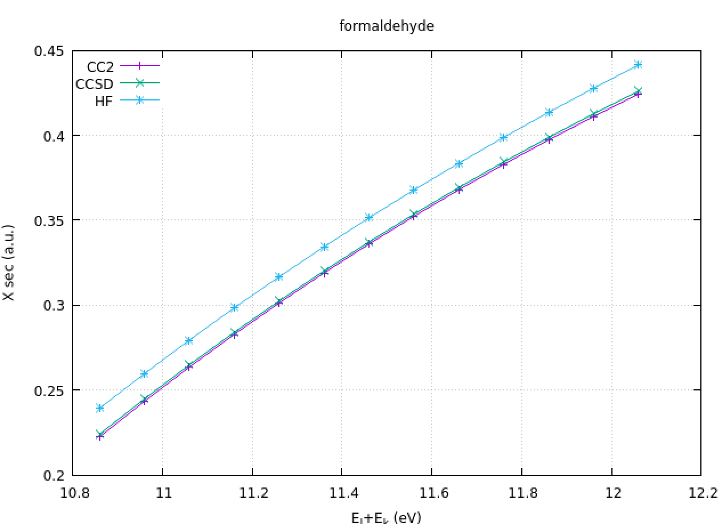
\includegraphics[width=0.6\textwidth]{chapters/appendix/image/Picture2.png}\\
\vfill
\clearpage

\vfill
\ch{OH-}, EE to IP [\ch{OH^{-*}} $\longrightarrow$ \ch{OH^{.}}], Basis set: 6-31G*
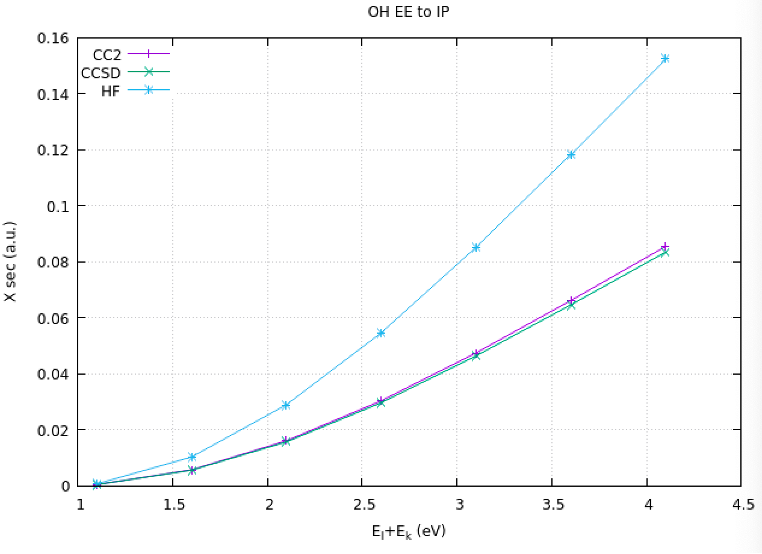
\includegraphics[width=0.6\textwidth]{chapters/appendix/image/OH-.png}\\
\vfill
\ch{NO}, EA($^2$B) -- GS [\ch{NO^*} $\longrightarrow$ \ch{NO+}], Basis set: aug-cc-pVTZ
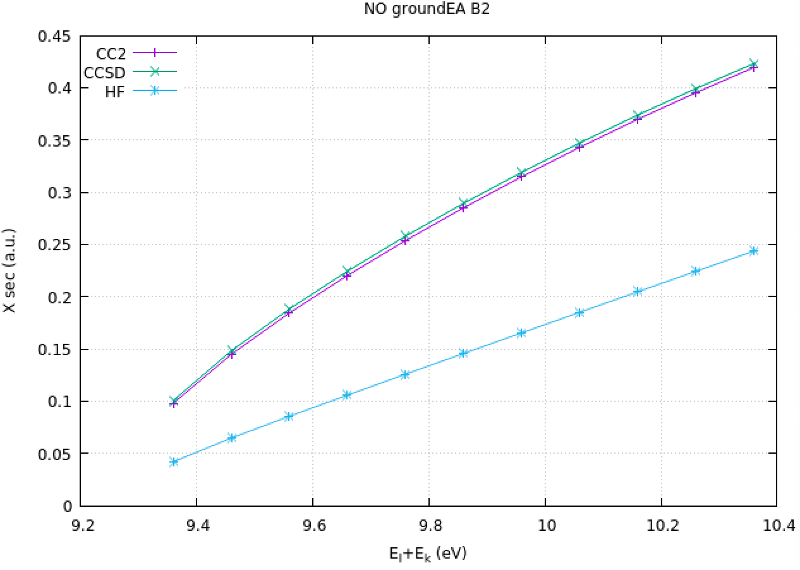
\includegraphics[width=0.6\textwidth]{chapters/appendix/image/NO.png}\\
\vfill
\ch{H2O}, GS(O 1s) -- IP [\ch{H2O} $\longrightarrow$ \ch{H2O^+}], Basis set: cc-pVTZ
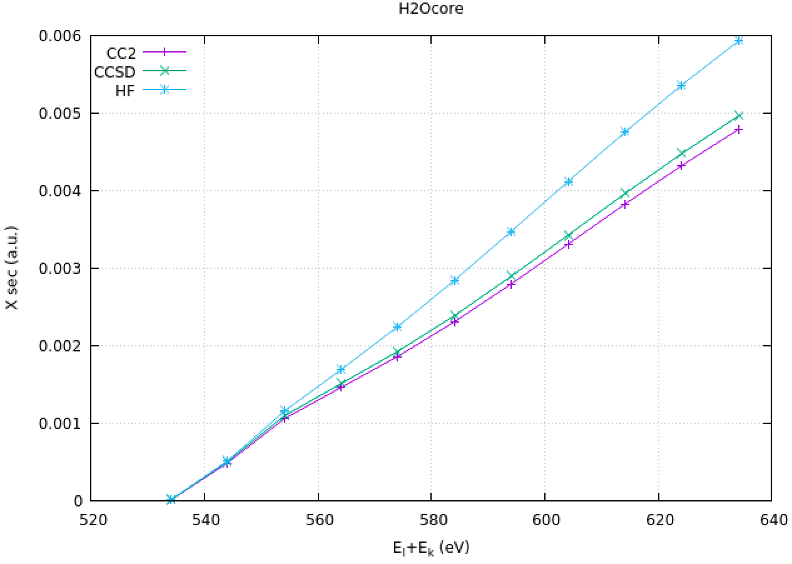
\includegraphics[width=0.6\textwidth]{chapters/appendix/image/H2O.png}\\
\vfill
\clearpage

\vfill
\ch{CO}, GS($^1$B or $^1$A) $\to$ IP [\ch{CO} $\longrightarrow$ \ch{CO^+}], Basis set: cc-pVDZ
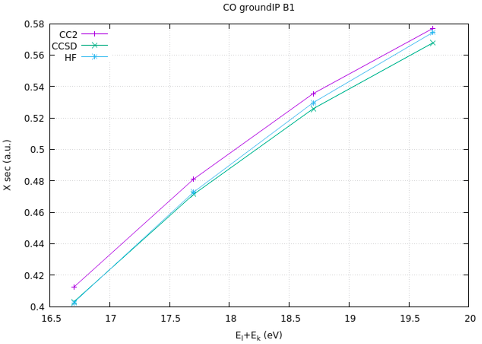
\includegraphics[width=0.5\textwidth]{chapters/appendix/image/CO1.png}
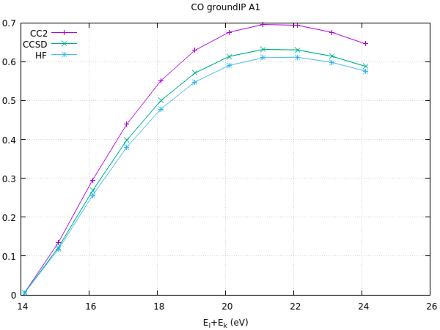
\includegraphics[width=0.49\textwidth]{chapters/appendix/image/CO2.png}\\
\vfill
\subsection*{Dipole-Bound Anions Photodetachment (aug-cc-pVTZ+6s3p)}
Acetone\\
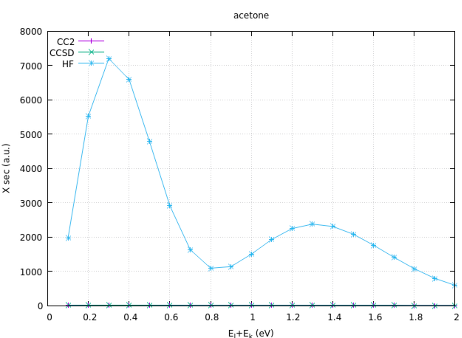
\includegraphics[width=0.49\textwidth]{chapters/appendix/image/Acetone1.png}
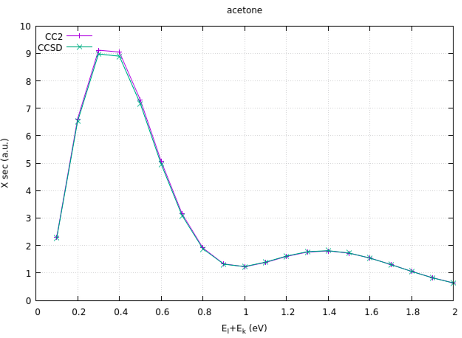
\includegraphics[width=0.49\textwidth]{chapters/appendix/image/Acetone2.png}\\
\vfill
Formamide\\
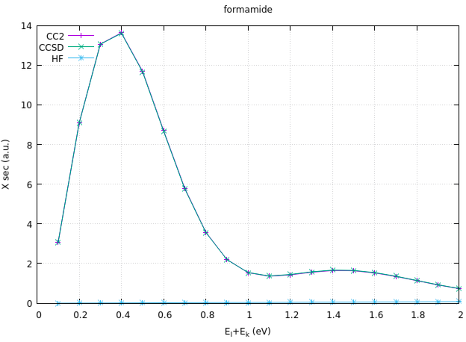
\includegraphics[width=0.48\textwidth]{chapters/appendix/image/Formamide1.png}
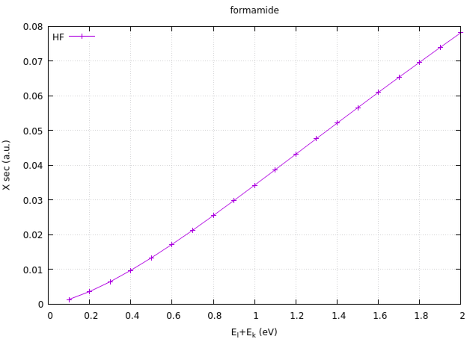
\includegraphics[width=0.48\textwidth]{chapters/appendix/image/Formamide2.png}\\
\vfill
\clearpage

\vfill
Nitrobenzene(DBS)\\
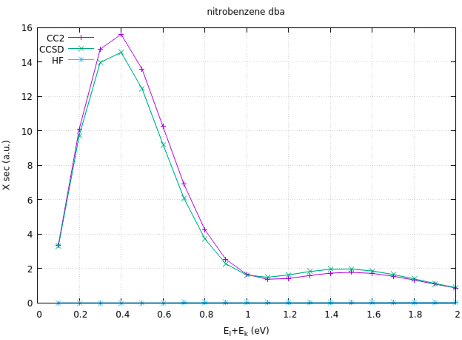
\includegraphics[width=0.49\textwidth]{chapters/appendix/image/Nitrobenzene1.png}
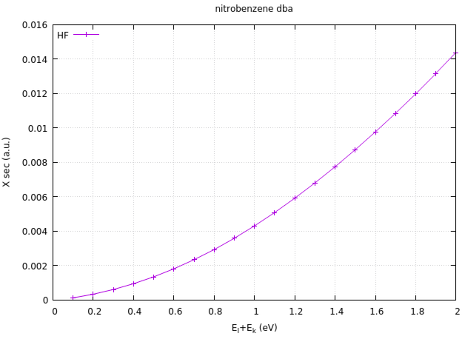
\includegraphics[width=0.49\textwidth]{chapters/appendix/image/Nitrobenzene2.png}\\
\vfill
\subsection*{Valence-Bound Anions Photodetachment (aug-cc-pVTZ)}
Benzoquinone\\
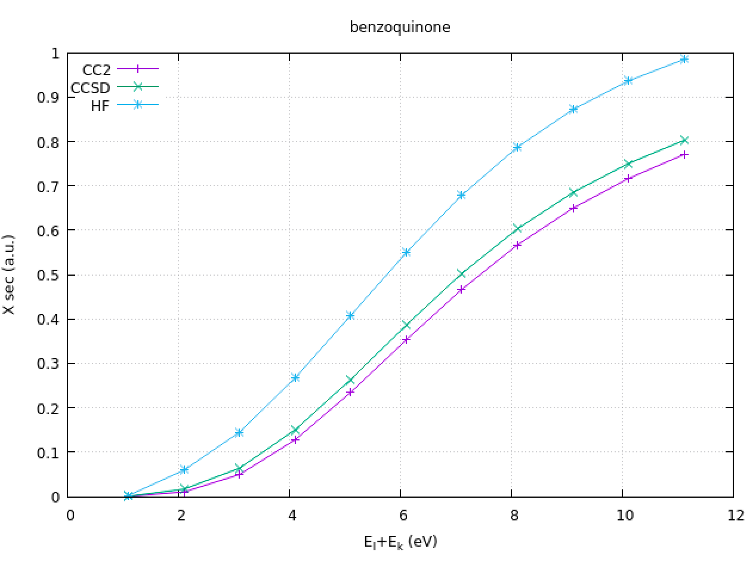
\includegraphics[width=0.6\textwidth]{chapters/appendix/image/benzoquinone.png}
\vfill
1,3-Dicyanobenzene\\
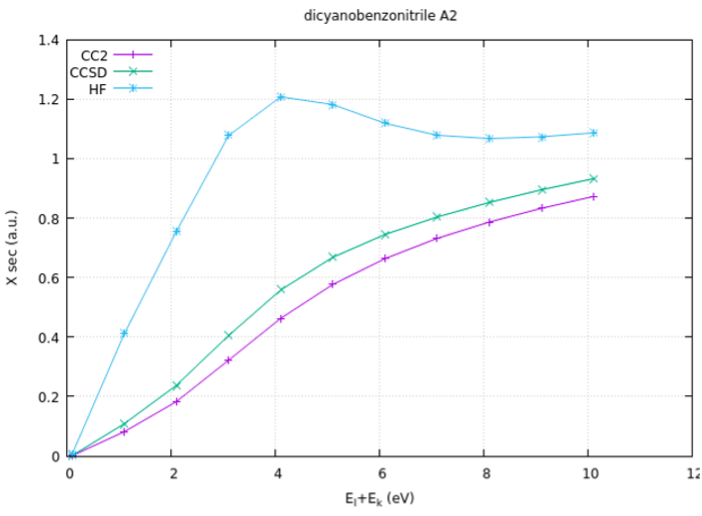
\includegraphics[width=0.49\textwidth]{chapters/appendix/image/diacyanobenzene1.png}
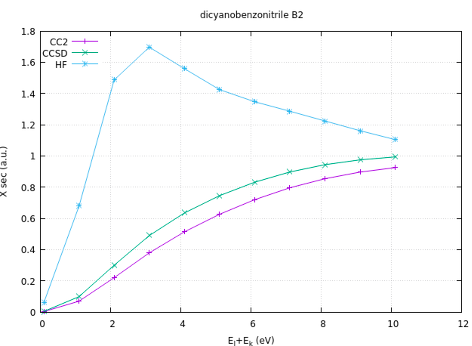
\includegraphics[width=0.49\textwidth]{chapters/appendix/image/diacyanobenzene2.png}\\
\vfill
\clearpage

\vfill
Maleic anhydride\\
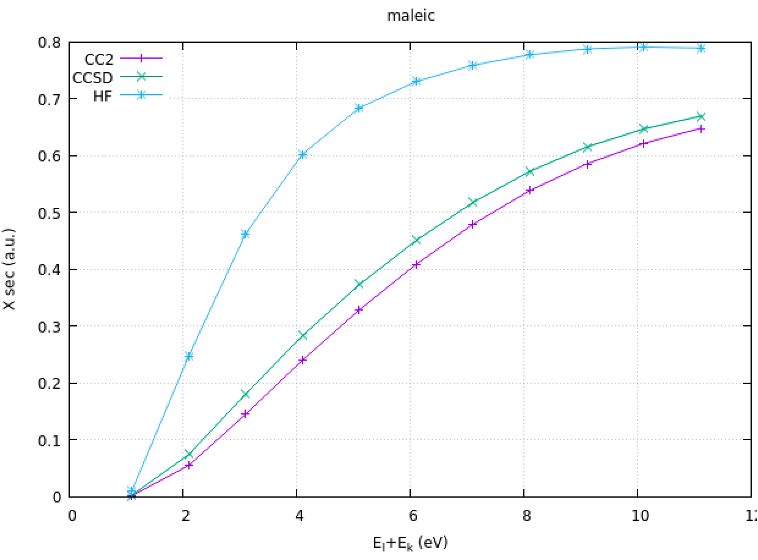
\includegraphics[width=0.6\textwidth]{chapters/appendix/image/maleic.png}
\vfill
Nitrobenzene(VBS)\\
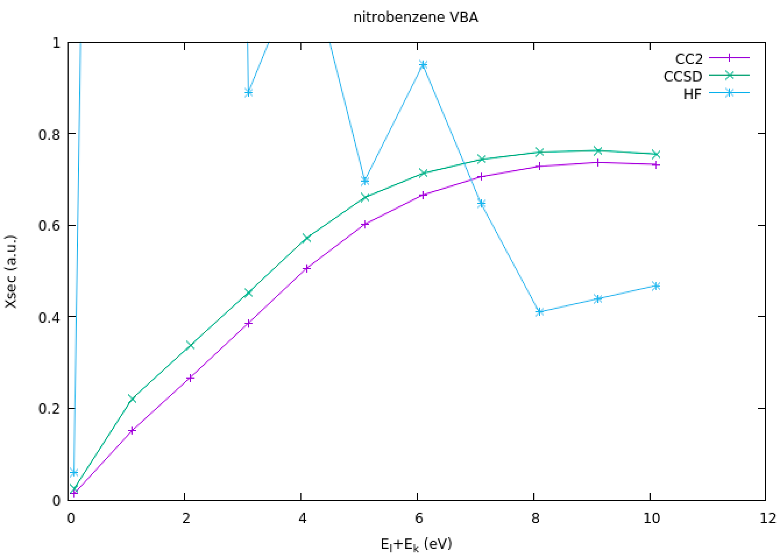
\includegraphics[width=0.6\textwidth]{chapters/appendix/image/nitrobenzeneVBA.png}\\
\vfill
Phenazine\\
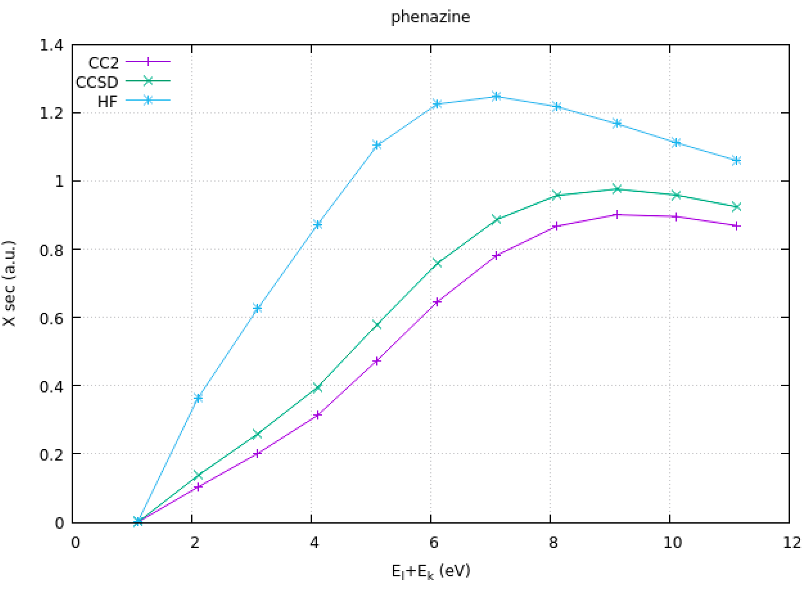
\includegraphics[width=0.6\textwidth]{chapters/appendix/image/phenazine.png}\\
\vfill




%%%%%%%%%%%%%%%%%%%%%%%%%%%%%%%%%%%%%%%%%%%%%%%%%%
% Keep the following \cleardoublepage at the end of this file, 
% otherwise \includeonly includes empty pages.
\cleardoublepage

% vim: tw=70 nocindent expandtab foldmethod=marker foldmarker={{{}{,}{}}}
